\documentclass{../template/texnote}

\title{\textbf{AI Models as Black Boxes: Not for Long}}[author={Linn Abraham}]

\begin{document}
    \maketitle \currentdoc{note}
    %<*note>

% Git is version control for your code. 
% Since code is mainly in the form of text files we can also say that Git is mainly version control for text data.
% Do not use try to use Git to version control binary data or other more non-text data.
% One reason is that the free cloud versions of Git like Github or Gitlab would not like to host big data in their servers for free.
% This also implies not to put your Jupyter notebook under version control. The diffs are not going to be readable unless you use specific software.




% \begin{itemize}
%     \item Git gives you the ability to take diffs.
%     \item Diffs give you the ability to patch.
%     \item Checkpoint the entire state of a directory and travel through time.
%     \item Allows you to keep a stable production ready version of your code at the same time working on different experiments to improve it.
%     \item Ability to collaborate simultaneously with other people.
%     \item Github gives you more advantages like shouting out to the world that this is your code.
%     \item A free backup of your work and checkpoints.
    
    
% \end{itemize}



% \section{Outline}
% \begin{enumerate}
%     \item Labelling data for supervised ML problems
%     \item Implementing specific models using code
%     \item Hyper-parameter tuning
%     \item Version controlling experiments
% \end{enumerate}

% \section{Version controlling your experiments}
% As a scientist it is often valuable to know how every step or action you are doing is helping with the end goal.
% In order to achieve this it is necessary to be systematic from the very beginning.
% Your code requires version controlling, comments, documentation and readme.
% Your data requires version control.
% Your hyperparameters need to be version controlled.
% Your model needs to be saved.
% Your training process need to give you feedback.
% Here you need to understand an overfit model from one that is not overfit.
% It is often advised to at least achieve an overfit model.

% \section{Data}
% Should you create your own dataset or use a pre-trained network?
% Or should you fine-tune a pre-trained network?
% Getting access to clean, labelled data is a crucial part of the ML project.
% Many a times it might be necessary to create data labels ourselves.
% For example if you want to convert an object detection problem to a segmentation problem.
% It might also be required to do some of the cleaning.
% What do you mean by data cleaning though?
% In terms of images, sometimes an image be noisy that makes it useless or misleading for the network.
% Some example of these are images with artefacts, poor resolution, small size of the object of interest etc.
% These can be termed bad images if you may.
% If all images of a particular class in your training set also has some associated artefact, the network may learn a non-existing correlation.
% Some of the image may be difficult, what I mean by this is that these may be rare kinds of a certain class etc. These are valuable.
% Since at this stage you might be messing with the real data, it might be worthwhile to think about when to create and keep apart a test set.
% How you would load the data depends on the size of your data and the amount of CPU RAM or GPU memory at your disposal. 
% Sometimes you might not have a balanced data set.
% What effects do these have?
% \subsection{Reading Data}
% The format of the data you might find would depend on the domain you are working in.
% In astronomy you might find that FITS is a common format. PNG or JPEG images are also common.
% It is worth knowing about why such different formats exist.
% How can you read and analyze such data?
% Python is a catch-all for all such data.
% But knowing other utitlies might also come in handy.
% For example, ImageJ, IRAF, TopCat, DS9, FitsViewer etc.
% A tool for labelling data is Label-Studio.
% \section{Hyper-parameter tuning}

% \begin{itemize}
%     \item Your dataset doesn't fit in your memory.
%     \item Your dataset is class imbalanced
% \end{itemize}

\section{Introduction}
It is quite common to hear the phrase that ``AI/ML models are black boxes". How true is this and is there any scope for the state-of-affairs to be improved? 
Before trying to understand this, a natural question might arise - Is there a problem if AI models remain black boxes as long as they work?
Let's try to answer this.



\textbf{Satisfying natural human curiosity.} Why do ML models work where traditional methods fail? Why do classical ML algorithms like random forest algorithms or SVMs show superior performance in certain areas where deep neural network fail to meet benchmarks?
All such questions stem from our natural curiosity to understand things.

\textbf{Adding to scientific knowledge.} If something works and one is not able to explain why it has worked. Then you might be adding nothing to the existing scientific knowledge.
However if the model works better than traditional approaches then this shows that the model has learnt something that other approaches have missed. Extracting this information out can be very useful to increase our understanding of the scientific problem.

\textbf{Improving existing models.}
Being able to understand the inner workings of the ML model allows to understand it's weakness and thus build a better model.

\textbf{Trust, Fairness and Privacy}
With the ever increasing integration of AI into our everday life, question of fairness naturally arise.
Even in our current scenarios of people making decision, its frustrating to be denied a loan when you are in dire need of it.
But imagine when the machines are doing the job and you desire to know why your loan request was denied.
Since ML models  are prone to the bias that exists in the data, can we trust such a model? How can fairness be programmed into the model? 
Similarly, privacy becomes a bigger concern if data that you provide is going to be used in a way that negatively affects you.


\begin{figure}[htpb]
    %\centering
    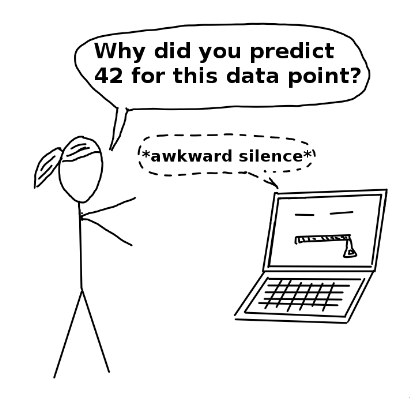
\includegraphics[width=0.35\textwidth]{Linn/comic.png}
    \caption{(Image Credit: Interpreatable Machine Learning by Christoph Molnar)}
    \label{fig:comic}
\end{figure}
\section{Towards Interpretable Machine Learning}

I hope that you are convinced that  ML models should be more than just black box algorithms that give better results on some metrics like classification accuracy or so. 
It is often the case that a single metric like classification accuracy is an incomplete description of most real-world tasks.
\cite{doshi-velez_towards_2017}.
\nocite{molnar_interpretable_2019}
The opposite of a black-box model might be a model that is said to be interpretable.
Interpretable Machine Learning refers to methods and models that make the behavior and predictions of machine learning systems understandable to humans.
It is currently an area of active research in Machine Learning.
But what does it actually mean to say that a model is interepretable?
There is no mathematical definition of interpretability. However when comparing two models, it could be said that a model is more interpretable than the other if it's decisions are easier for a human to understand.
What are the ways in which interpretability can be incorporated into machine learning?

\textbf{Algorithm Transparency.} How does the algorithm learn a model from the data and what kind of relationships are learned from it?
People with experience in Convolutional Neural Networks  (CNN) know that the lowest layers of a CNN learn edge detectors.
The least squares method, a kind of linear model, also is a method where the working of the algorithm is known.

\textbf{Global Model Interpretability.}
This involves knowing the entire model at once.
To explain the model output on a global level requires you to explain the trained model, the algorithm and the data involved.

\textbf{Global Model Interpretability on a Modular Level}
A Naive Bayes model with many hundreds of features would be too big for me and you to keep in our working memory.
To predict what the output would be given a data point would be near impossible without actually computation.
But what you can do is try to comprehend the impact of a single weight.

\textbf{Local Interpretability for a Single Prediction}
You can zoom in on a single instance and examine what the model predicts for this input, and explain why.

%\section*{What is an Explanation?}
%Although we have been requiring that the model be explainable what is the property of an explainable or interpretable model?
%%\textbf{What is an explanation?}. 
%An explanation is said to be the answer to a why-question.
%Questions that start with a ``Why'' can usually be substituted for a  ``How'' question and vice-versa.
%If someone asks you, ``Why is the water boiling?''. You could impress upon them that the once the vapour pressure and atmospheric pressure equals the water has no choice but to boil. And this means that the bulk process of phase change has to start and temperature remains constant while this is happening.
%In effect you are answering the question ``How boiling happens''.
%(One could also answer the same question by saying that ``It is boiling because I want to make coffee''.
%That is if you are asking what the human centric purpose behind the event is.)

\section{A survey of existing interpretability methods}
%\section*{Interpretable Models}
\textbf{Interpretable Models.} Linear regression, logistic regression, decision trees, Support Vector Machines are some of the easily interpretable machine learning models.
There are several methods that are focussed on such easily interpretable and linear methods.


\textbf{Model-Agnostic Methods.} Such methods have several advantages over methods are specifically designed based on the model. Better comparisons can be done as the same methods 
is used to evaluated different models. Also model specific methods are much more rigid in comparison to model agnostic ones.
The alternative to using model-agnostic methods is to only use interepretable models which may not be ideal in all scenarios.
Let us take a high level look at model-agnostic interpretability.
We capture information about the world by collecting data. 
It is then abstracted by learning to predict the data for a specific task using a black-box ML model.
Interpretability is then another layer on top of this that helps human understand the black-box model.

\begin{figure}[htpb]
    \centering
    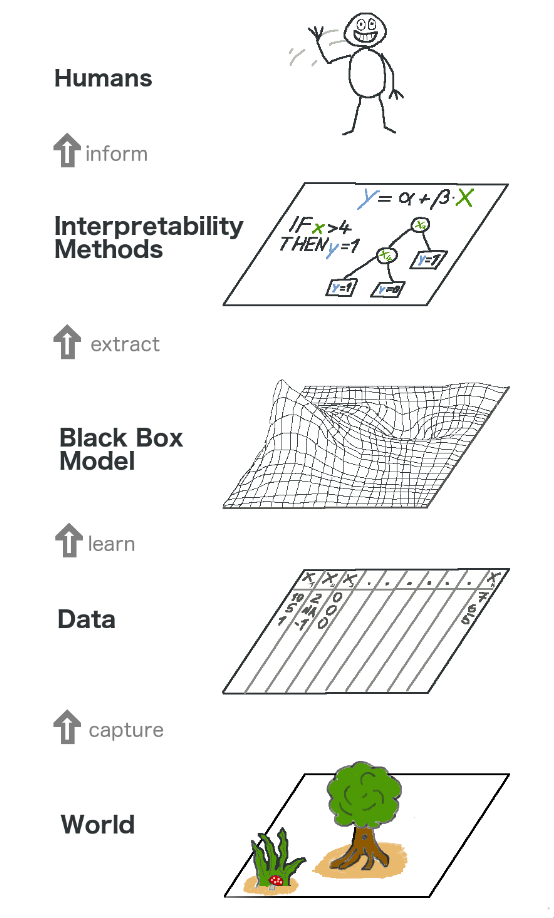
\includegraphics[width=0.55\textwidth]{Linn/bigpic.png}
    \caption{A graphic showing the big picture of explainable machine learning. (Image Credit: Interpreatable Machine Learning by Christoph Molnar}
    \label{fig:bigpic}
\end{figure}



There are several model-agnostic methods that are worth mentioning. 
LIME or Local Interpretable Model Agnostic Explanations \cite{doshi-velez_towards_2017} is one such method. 
Another one is analyzing Shapley values.
We will be going into detail into both these methods in the upcoming issue.

\textbf{Example-Based methods.} These can be considered model-agnostic as they make any machine learning model more interpretable. 
These are different from the other methods in they select data instances and do not make use of the feature summaries or feature importance.
Such methods can be motivated with examples from daily life. 
Doctors in their clinical practice often uses patients who have had similar symptomps in order to make diagnosis.
Another example might be a gamer who makes decision based on gameplays with similar situations he had encountered in the past.
The template for such explanations is based on the following.
Thing B is similar to thing A and A caused Y, so I predict that B will cause Y as well.
Some machine learning models are implicitly example based such as decision trees. 
For a new instance, a knn model locates the k-nearest neighbors and returns the average of the outcomes of those neighbors as a prediction.

There are several example-based methods that can be used.
\begin{enumerate}
\item \textbf{Counterfactual explanations} tell us how an instance has to change to significantly change its prediction.
\item \textbf{Adversarial examples} are counterfactuals used to fool machine learning models. The emphasis is on flipping the prediction and not explaining it.
\item \textbf{Prototypes} are a selection of representative instances from the data and criticisms are instances that are not well represented by those prototypes.
\item \textbf{Influential instances} are the training data points that were the most influential for the parameters of a prediction model or the predictions themselves.
\end{enumerate}

\begin{figure}[htpb]
    \centering
    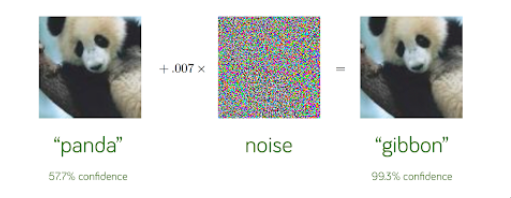
\includegraphics[width=0.85\textwidth]{Linn/panda.png}
    \caption{A classic example of an adversarial attack that that causes a CNN to misclassify a panda as a gibbon. This is a mistake that a human would never make. (Image Credit: Interpreatable Machine Learning by Christoph Molnar)}
    \label{fig:panda}
\end{figure}



\textbf{Neural Network Interpretation methods.} There are several interpretation methods that are specific to neural networks. 
The different categories of techniques that fall under this are:
\begin{enumerate}
    \item \textbf{Feature Visualization:} Visualizing what features the network has learned.
    \item \textbf{Concepts:} Which abstract concepts has the neural network learned?
    \item \textbf{Feature Attribution:} These try to explain how each input feature contributed to a particular prediction.
    \item \textbf{Model distillation:} This attempts to explain a neural network using a simpler model.
\end{enumerate}

\textbf{Pixel Attribution} can be seen as a special case of feature attribution but for images.
It is known under various names such as sensitivity map, saliency map, pixel attribution map, gradient-based attribution methods, feature relevance, feature attribution, and feature contribution.
Pixel attribution methods can be classified based on several criteria.
\begin{enumerate}
    \item  There are \textbf{occlusion or perturbation} based methods. Methods such as SHAP and LIME fall under these.
These change parts of the image in order to generate explanations.
\item  \textbf{Gradient-based} methods compute the gradient of the prediction with respect to the input features.
There are several gradient based methods that differ in the way the gradient is computed.

\end{enumerate}
What is common to both the methods is that the explanation and the input image are of the same size or shape. 
And each pixel is assigned a value that highlights its importance towards the prediction.

Another distinction can be made within pixel attribution methods based on the baseline question.
\begin{enumerate}
    \item \textbf{Gradient-only} methods tell us whether a change in pixel would cause the model prediction to change.
        Examples are Vanilla Gradient and Grad-CAM.
    \item \textbf{Path-attribution} methods compare the input image to a reference image or a baseline image. This is usually taken to be a black image (a "zero" image).
        This includes methods such as integrated gradients, as well as the methods such as LIME and SHAP.
Some path attribution methods are "complete", meaning that the sum of the relevance values for all input features is the difference between the prediction of the image minus the prediction of a reference image.
The difference between classification scores of the actual image and the baseline image are attributed to the pixels. The choice of the reference image (distribution) has a big effect on the explanation.
\end{enumerate}

\begin{figure}[htpb]
    \centering
    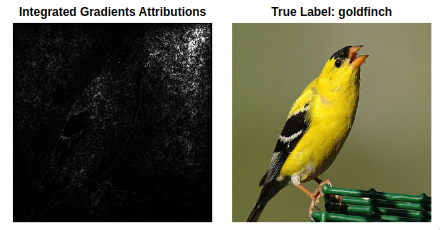
\includegraphics[width=0.65\textwidth]{Linn/goldfinch.png}
    \caption{Pixel-wise attributions of the Inception V4 network using integrated gradients. Notice that the grey background of the image has higher attributions than more relevant pixels.(Image Credit: Interpreatable Machine Learning by Christoph Molnar)}
    \label{fig:goldfinch}
\end{figure}

%\textbf{Intrinsic or Post-Hoc.} Some models such as decision-trees are intrinsically interpretable whereas neural networks are not.
%Examples of machine learning models that are interpretable are decision trees, SVM, linear regression etc.
%Neural networks are not very easily interpretable. However there exists methods to extract interpretations out of the trained model.

%\textbf{Model specific or model agnostic.}
%The interpretation of regression weights in a linear model is a model-specific interpretation, since -- by definition -- the interpretation of intrinsically interpretable models is always model-specific.
%Model-agnostic tools can be used on any machine learning model and are applied after the model has been trained (post hoc).

%\textbf{Local or Global.}
%Does the interpretation method explain an individual prediction or the entire model behavior?

%In the coming issue we will be looking to specific interpretability models namely, LIME (Local Interpretable Model Agnostic Explanations) and Shapley values.
\nocite{lipton_mythos_2017}
\nocite{miller_explanation_2018}

\begin{thebibliography}{}

\bibitem[{Doshi-Velez} and Kim(2017)]{doshi-velez_towards_2017}
Finale {Doshi-Velez} and Been Kim.
\newblock Towards {{A Rigorous Science}} of {{Interpretable Machine Learning}},
  March 2017.

\bibitem[Molnar(2019)]{molnar_interpretable_2019}
Christoph Molnar.
\newblock \emph{Interpretable Machine Learning: A Guide for Making {{Black Box
  Models}} Interpretable}.
\newblock {Lulu}, {Morisville, North Carolina}, 2019.
\newblock ISBN 978-0-244-76852-2.

\bibitem[Lipton(2017)]{lipton_mythos_2017}
Zachary~C. Lipton.
\newblock The {{Mythos}} of {{Model Interpretability}}, March 2017.

\bibitem[Miller(2018)]{miller_explanation_2018}
Tim Miller.
\newblock Explanation in {{Artificial Intelligence}}: {{Insights}} from the
  {{Social Sciences}}, August 2018.

\end{thebibliography}


% \end{thebibliography}

\vspace{0.5cm}
\noindent\fbox{%
	\parbox{\textwidth}{%
		\textbf{About the Author}\vspace{0.2cm} \\
		\textbf{Linn Abraham} is a researcher in Physics, specializing in A.I. applications to astronomy. He iscurrently involved in the development of CNN based Computer Vision tools for classifications of astronomicalsources from PanSTARRS optical images. He has used data from a several large astronomical surveys includingSDSS, CRTS, ZTF and PanSTARRS for his research.
		
	}
}
    %</note>
    \printbibliography
\end{document}
